\documentclass[../../main.tex]{subfiles}

\graphicspath{{../../image/}{../../figure/}}

\begin{document}

\section{周期变量}\label{section:ch03-周期变量}

尽管 Gauss 分布本身具有重要的实际意义，并且作为构建更复杂概率模型的基础也十分有用，但在某些情况下，它们并不适合作为连续变量的密度模型。实际应用中存在的周期变量就属于这种情况。

特定地理位置的风向是周期变量的一个例子。例如，我们在测量多个地理位置的风向后，希望使用参数分布来总结这些数据。另一个例子是日历时间，我们想建模那些可能在 24 小时或一年内具有周期性的量。这样的量可以使用 $0\leqslant\theta<2\pi$ 范围内的角（极）坐标来方便地表示。

我们可以选择某个方向作为起始方向，然后应用 Gauss 分布等常规分布来处理周期变量。然而，这种方法所产生的结果极其依赖于我们随意选择的起始方向。例如，假设有两个观测值 $\theta_1=1^{\circ}$ 和 $\theta_2=359^{\circ}$，并且我们使用标准的单元 Gauss 分布对它们建模。如果将起始方向设置为 $0^{\circ}$，那么该数据集的样本均值为 $180^{\circ}$，标准差为 $179^{\circ}$；而如果将起始方向设置为 $180^{\circ}$，那么该数据集的样本均值为 $0^{\circ}$，标准差为 $1^{\circ}$。显然，我们需要一种专门用来处理周期变量的方法。

考虑估计周期变量 $\theta$ 的一组观测值 $\mathcal{D}=\{\theta_1,\cdots,\theta_N\}$ 的均值，其中 $\theta$ 的单位为弧度。简单计算均值 $(\theta_1+\cdots+\theta_N)/N$ 将与坐标系强相关。为了找到均值的不变度量，我们注意到观测值可以视为单位圆上的点，因此可以用二维单位向量 $\boldsymbol{x}_1,\cdots,\boldsymbol{x}_N$ 来描述它们，其中对于 $\boldsymbol{x}_1,\cdots,\boldsymbol{x}_N$，$\lVert\boldsymbol{x}_n\rVert=1$，如\cref{figure:ch03-圆周均值}所示。对向量 $\{\boldsymbol{x}_n\}$ 求平均值，可得
\begin{align}
\bar{\boldsymbol{x}}=\frac{1}{N}\sum_{n=1}^{N}\boldsymbol{x}_n,\qquad \boldsymbol{x}_n=(\cos\theta_n,\sin\theta_n)^{\mathsf{T}}.
\label{align:ch03-周期均值向量}
\end{align}

\begin{definition}[圆周均值]\label{definition:ch03-圆周均值}
设 $\theta_1,\cdots,\theta_N$ 为周期变量的观测值，$\boldsymbol{x}_n=(\cos\theta_n,\sin\theta_n)^{\mathsf{T}}$。称由\eqref{align:ch03-周期均值向量}给出的 $\bar{\boldsymbol{x}}$ 的平均方向所对应的角度 $\bar{\theta}$ 为这组观测值的圆周均值（circular mean），其中 $\bar{\boldsymbol{x}}=\bar{r}(\cos\bar{\theta},\sin\bar{\theta})^{\mathsf{T}}$，$\bar{r}\geqslant0$。
\end{definition}

% SUPPLEMENT: parent=definition:ch03-圆周均值; kind=motivation; location=紧随其后的 remark（重构新增）
\begin{remark}（重构新增）
引入圆周均值的目的是消除“起始方向”这一人为选择的影响：把角度换成单位圆上的点之后再平均，结果就与 $0^{\circ}$ 定在哪里无关。这正是开头“$1^{\circ}$ 与 $359^{\circ}$”例子的解药——按向量平均，两个几乎重合的点会给出接近 $0^{\circ}$ 的均值，而不是荒谬的 $180^{\circ}$。

定义中的 $\bar{r}$ 称为平均合成长度（resultant length），它度量观测在圆周上的集中程度：$\bar{r}\approx1$ 表示方向高度一致，$\bar{r}\approx0$ 表示方向弥散。只有当 $\bar{\boldsymbol{x}}\neq\boldsymbol{0}$ 时 $\bar{\theta}$ 才唯一确定；若 $\bar{\boldsymbol{x}}=\boldsymbol{0}$（例如两个方向正好相反），则均值方向无定义，这是与实数均值的重要区别。
\end{remark}

\begin{figure}[htbp]
  \centering
  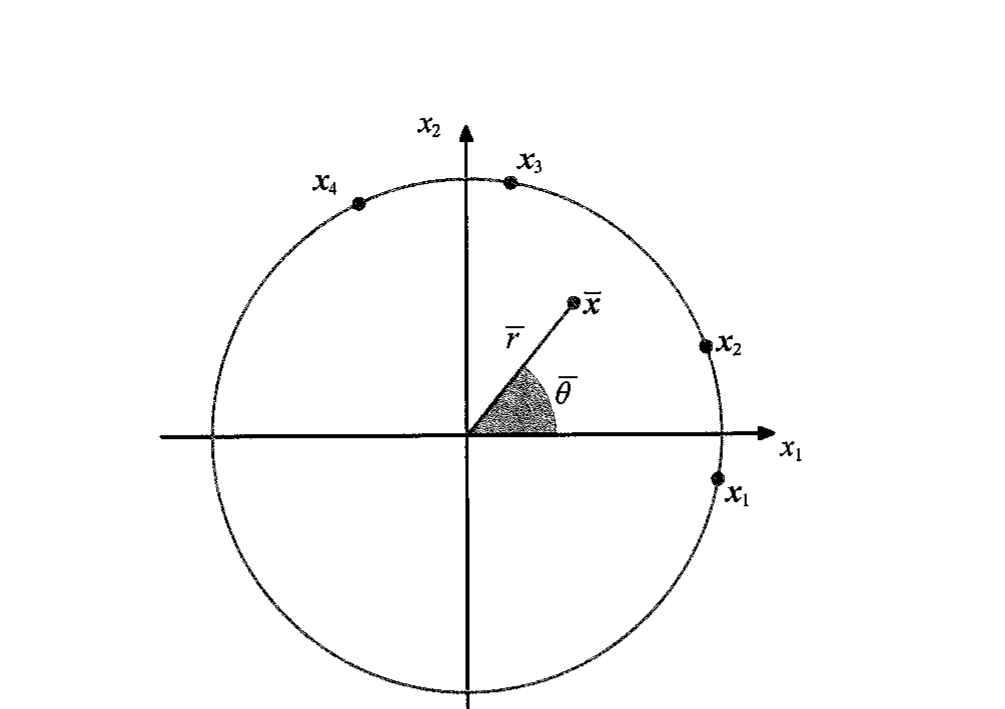
\includegraphics[width=0.62\textwidth]{ch03-fig3-9-circular-mean.png}
  \caption{将周期变量的值 $\theta_n$ 表示为位于单位圆上的二维向量 $\boldsymbol{x}_n$ 的示意图，同时还展示了这些向量的平均值 $\bar{\boldsymbol{x}}$。}
  \label{figure:ch03-圆周均值}
\end{figure}

然后找到与平均值对应的角度 $\bar{\theta}$。显然，上述定义将确保均值的位置与角坐标的起始方向无关。注意 $\bar{\boldsymbol{x}}$ 通常位于单位圆内。观测值的笛卡儿坐标由 $\boldsymbol{x}_n=(\cos\theta_n,\sin\theta_n)$ 给出，样本均值的笛卡儿坐标可以写成 $\bar{\boldsymbol{x}}=(\bar{r}\cos\bar{\theta},\bar{r}\sin\bar{\theta})$。代入\eqref{align:ch03-周期均值向量}并使 $x_1$ 和 $x_2$ 分量相等，则有
\begin{align}
\bar{x}_1=\bar{r}\cos\bar{\theta}=\frac{1}{N}\sum_{n=1}^{N}\cos\theta_n,\qquad \bar{x}_2=\bar{r}\sin\bar{\theta}=\frac{1}{N}\sum_{n=1}^{N}\sin\theta_n.
\label{align:ch03-周期分量}
\end{align}
对二者取比值，并使用恒等式 $\tan\theta=\sin\theta/\cos\theta$，$\bar{\theta}$ 可由下式求解：
\begin{align}
\bar{\theta}=\tan^{-1}\!\left(\frac{\sum_n\sin\theta_n}{\sum_n\cos\theta_n}\right).
\label{align:ch03-周期均值角}
\end{align}

\begin{proposition}[圆周均值的显式表达]\label{proposition:ch03-圆周均值公式}
设 $\bar{\boldsymbol{x}}\neq\boldsymbol{0}$，则圆周均值 $\bar{\theta}$ 由\eqref{align:ch03-周期均值角}给出（按象限取 $\tan^{-1}$ 的相应分支），且它不依赖于角坐标起始方向的选择。
\end{proposition}
\begin{proof}
（重构新增）由\eqref{align:ch03-周期分量}，$\bar{r}\cos\bar{\theta}=\frac1N\sum_n\cos\theta_n$、$\bar{r}\sin\bar{\theta}=\frac1N\sum_n\sin\theta_n$。由于 $\bar{\boldsymbol{x}}\neq\boldsymbol{0}$ 意味着 $\bar{r}>0$，两式相除得
\begin{align*}
\tan\bar{\theta}=\frac{\bar{r}\sin\bar{\theta}}{\bar{r}\cos\bar{\theta}}=\frac{\sum_n\sin\theta_n}{\sum_n\cos\theta_n},
\end{align*}
按象限取分支即得\eqref{align:ch03-周期均值角}。

至于与起始方向无关：若把起始方向旋转 $\alpha$，则每个观测变为 $\theta_n+\alpha$，对应向量变为 $\boldsymbol{R}_\alpha\boldsymbol{x}_n$（$\boldsymbol{R}_\alpha$ 为旋转矩阵），于是 $\bar{\boldsymbol{x}}$ 变为 $\boldsymbol{R}_\alpha\bar{\boldsymbol{x}}$，其方向角变为 $\bar{\theta}+\alpha$。可见均值随坐标系同步旋转，即相对位置不变。
\end{proof}

% SUPPLEMENT: parent=proposition:ch03-圆周均值公式; kind=motivation; location=紧随其后的 remark（重构新增）
\begin{remark}（重构新增）
\eqref{align:ch03-周期均值角}与普通的“算术平均”有本质区别：它不是角度的线性平均，而是先映射到单位圆、再平均、再取角度。这一“映射—平均—反映射”的模式在周期数据分析中普遍适用（例如周期数据的方差、相关系数都如此定义）。

公式\eqref{align:ch03-周期均值角}只给出比值，因此必须结合 $\sum_n\cos\theta_n$ 与 $\sum_n\sin\theta_n$ 的符号确定象限，否则会相差 $\pi$。当分母 $\sum_n\cos\theta_n=0$ 时比值无定义，此时 $\bar{\theta}=\pm\pi/2$，应由 $\bar{x}_1=0$ 与 $\bar{x}_2$ 的符号直接判定。
\end{remark}

读者很快就会看到这个结果是如何作为最大似然估计量而产生的。

按照惯例，考虑分布 $p(\theta)$，其具有 $2\pi$ 周期。任何定义在 $\theta$ 上的概率密度 $p(\theta)$ 都必须是非负的且积分等于 $1$，同时还必须具有周期性。因此，$p(\theta)$ 必须满足以下 3 个条件：
\begin{align}
p(\theta)\geqslant0,
\label{align:ch03-周期分布非负}
\end{align}
\begin{align}
\int_{0}^{2\pi}p(\theta)\,\mathrm{d}\theta=1,
\label{align:ch03-周期分布归一}
\end{align}
\begin{align}
p(\theta+2\pi)=p(\theta).
\label{align:ch03-周期分布周期}
\end{align}

\begin{definition}[周期分布]\label{definition:ch03-周期分布}
设 $p(\theta)$ 为定义在实轴上的非负函数，若它满足\eqref{align:ch03-周期分布非负}至\eqref{align:ch03-周期分布周期}，则称 $p(\theta)$ 为周期分布（或圆周分布）的密度。
\end{definition}

% SUPPLEMENT: parent=definition:ch03-周期分布; kind=motivation; location=紧随其后的 remark（重构新增）
\begin{remark}（重构新增）
这三个条件把“概率密度”与“周期性”两件事同时固定下来：前两条是密度的通用要求，第三条是周期变量特有的要求。有了第三条，$p$ 就可以看作定义在单位圆上的函数，因此“把实轴上的分布卷到圆周上”这种构造才有意义。

注意积分区间取 $[0,2\pi)$ 即可，周期性保证了在任意长度为 $2\pi$ 的区间上积分都相同。由\eqref{align:ch03-周期分布周期}还可推出，对任何整数 $M$ 有 $p(\theta+2M\pi)=p(\theta)$，这说明圆周上的每一点都对应实轴上无穷多个等价点，也解释了为什么周期分布不能直接沿用实轴上的矩（平均值、方差）概念。
\end{remark}

从\eqref{align:ch03-周期分布周期}可知，对于任何整数 $M$，$p(\theta+2M\pi)=p(\theta)$。

我们可以很容易地获得满足上述 3 个条件的类 Gauss 分布：考虑二元变量 $\boldsymbol{x}=(x_1,x_2)$ 上的 Gauss 分布，其均值为 $\boldsymbol{\mu}=(\mu_1,\mu_2)$，协方差矩阵为 $\boldsymbol{\Sigma}=\sigma^{2}\boldsymbol{I}$，其中 $\boldsymbol{I}$ 是 $2\times2$ 的单位矩阵，故有
\begin{align}
p(x_1,x_2)=\frac{1}{2\pi\sigma^{2}}\exp\left\{-\frac{(x_1-\mu_1)^{2}+(x_2-\mu_2)^{2}}{2\sigma^{2}}\right\}.
\label{align:ch03-二维Gauss}
\end{align}
常数 $p(\boldsymbol{x})$ 的等值线为圆形，如\cref{figure:ch03-冯米塞斯几何}所示。

\begin{figure}[htbp]
  \centering
  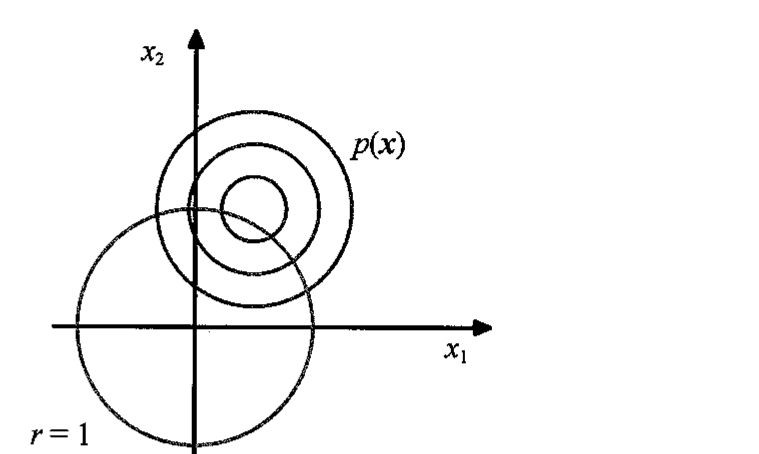
\includegraphics[width=0.45\textwidth]{ch03-fig3-10-vonmises-geom.png}
  \caption{von Mises 分布可通过\eqref{align:ch03-二维Gauss}所示的二维 Gauss 分布导出。图中蓝色的圆是其密度等值线，红色的单位圆是其条件。}
  \label{figure:ch03-冯米塞斯几何}
\end{figure}

考虑沿着固定半径的圆来取这个分布上的值。通过这种构造方法，尽管没有被归一化，但这个分布仍将是周期性的。我们可以通过从笛卡儿坐标 $(x_1,x_2)$ 转换到极坐标 $(r,\theta)$ 来确定该分布的形式：
\begin{align}
x_1=r\cos\theta,\qquad x_2=r\sin\theta.
\label{align:ch03-极坐标}
\end{align}
同时将均值 $\boldsymbol{\mu}$ 也映射到极坐标：
\begin{align}
\mu_1=r_0\cos\theta_0,\qquad \mu_2=r_0\sin\theta_0.
\label{align:ch03-极坐标均值}
\end{align}
接下来，我们设单位圆 $r=1$，将这些变换代入二维 Gauss 分布\eqref{align:ch03-二维Gauss}，以研究该分布与 $\theta$ 的依赖关系。关注 Gauss 分布中的指数部分，则有
\begin{align}
&-\frac{1}{2\sigma^{2}}\Bigl\{(r\cos\theta-r_0\cos\theta_0)^{2}+(r\sin\theta-r_0\sin\theta_0)^{2}\Bigr\}\nonumber\\
&\quad=-\frac{1}{2\sigma^{2}}\Bigl\{1+r_0^{2}-2r_0\cos\theta\cos\theta_0-2r_0\sin\theta\sin\theta_0\Bigr\}\nonumber\\
&\quad=\frac{r_0}{\sigma^{2}}\cos(\theta-\theta_0)+\text{const},
\label{align:ch03-指数极坐标}
\end{align}
其中“const”表示独立于 $\theta$ 的常数项。此处的推导使用了以下三角恒等式：
\begin{align}
\cos^{2}A+\sin^{2}A=1,
\label{align:ch03-三角恒等式1}
\end{align}
\begin{align}
\cos A\cos B+\sin A\sin B=\cos(A-B).
\label{align:ch03-三角恒等式2}
\end{align}
如果定义 $m=r_0/\sigma^{2}$，则可以得到 $p(\theta)$ 沿单位圆 $r=1$ 这个分布的最终表达式，形式为
\begin{align}
p(\theta\mid\theta_0,m)=\frac{1}{2\pi I_0(m)}\exp\bigl\{m\cos(\theta-\theta_0)\bigr\}.
\label{align:ch03-冯米塞斯分布}
\end{align}

\begin{theorem}[von Mises 分布]\label{theorem:ch03-冯米塞斯分布}
设 $p(\theta)$ 为单位圆上的周期密度，它由二维各向同性 Gauss 分布\eqref{align:ch03-二维Gauss}限制在 $r=1$ 上得到。则 $p(\theta)$ 具有\eqref{align:ch03-冯米塞斯分布}的形式，其中 $\theta_0$ 为均值方向，$m=r_0/\sigma^{2}>0$，归一化系数为
\begin{align}
I_0(m)=\frac{1}{2\pi}\int_{0}^{2\pi}\exp\{m\cos\theta\}\,\mathrm{d}\theta.
\label{align:ch03-修正Bessel函数}
\end{align}
\end{theorem}
\begin{proof}
（重构新增）把\eqref{align:ch03-极坐标}与\eqref{align:ch03-极坐标均值}代入\eqref{align:ch03-二维Gauss}并取 $r=1$，得
\begin{align*}
p(\theta)\propto\exp\left\{-\frac{1}{2\sigma^{2}}\Bigl[(r\cos\theta-r_0\cos\theta_0)^{2}+(r\sin\theta-r_0\sin\theta_0)^{2}\Bigr]\right\}_{r=1}.
\end{align*}
展开括号内的平方和：
\begin{align*}
&\cos^{2}\theta-2r_0\cos\theta\cos\theta_0+r_0^{2}\cos^{2}\theta_0+\sin^{2}\theta-2r_0\sin\theta\sin\theta_0+r_0^{2}\sin^{2}\theta_0\\
&\quad=1+r_0^{2}-2r_0(\cos\theta\cos\theta_0+\sin\theta\sin\theta_0)=1+r_0^{2}-2r_0\cos(\theta-\theta_0),
\end{align*}
其中用到\eqref{align:ch03-三角恒等式1}与\eqref{align:ch03-三角恒等式2}。于是
\begin{align*}
p(\theta)\propto\exp\left\{\frac{r_0}{\sigma^{2}}\cos(\theta-\theta_0)\right\}\exp\left\{-\frac{1+r_0^{2}}{2\sigma^{2}}\right\}\propto\exp\{m\cos(\theta-\theta_0)\},
\end{align*}
第二步把与 $\theta$ 无关的常数并入比例常数，并令 $m=r_0/\sigma^{2}$。这就是\eqref{align:ch03-指数极坐标}。

最后确定归一化常数。由于 $\cos(\theta-\theta_0)$ 关于 $\theta$ 以 $2\pi$ 为周期，故 $\int_0^{2\pi}\exp\{m\cos(\theta-\theta_0)\}\,\mathrm{d}\theta=\int_0^{2\pi}\exp\{m\cos\theta\}\,\mathrm{d}\theta=2\pi I_0(m)$，其中 $I_0(m)$ 由\eqref{align:ch03-修正Bessel函数}定义。因此归一化后的密度为
\begin{align*}
p(\theta\mid\theta_0,m)=\frac{1}{2\pi I_0(m)}\exp\{m\cos(\theta-\theta_0)\},
\end{align*}
即\eqref{align:ch03-冯米塞斯分布}。由于被积函数严格为正，$I_0(m)>0$，归一化常数良定义。
\end{proof}

% SUPPLEMENT: parent=theorem:ch03-冯米塞斯分布; kind=motivation; location=紧随其后的 remark（重构新增）
\begin{remark}（重构新增）
这一定理说明 von Mises 分布不是凭空构造的，而是“二维各向同性 Gauss 分布限制在单位圆上”的自然结果：Gauss 分布在平面上是单峰、等向的，切到单位圆上就得到圆周上的单峰分布，峰值方向由 $\boldsymbol{\mu}$ 的极角 $\theta_0$ 决定，峰的尖锐程度由 $m=r_0/\sigma^{2}$ 决定。

推导中有两个关键步骤：一是把 $r$ 固定为 $1$（只关心单位圆上的值），二是把与 $\theta$ 无关的因子并入归一化常数。注意这里得到的密度是关于 $\theta$ 的，而不是关于弧长的“密度乘以 $r$”；取 $r=1$ 恰好使二者一致。若取其他半径，得到的函数仍是周期的，但归一化常数会依赖 $r$。
\end{remark}

这称为 von Mises 分布或圆形正态（circular normal）分布。这里的参数 $\theta_0$ 对应于分布的均值，$m$ 则称为聚焦（concentration）参数，类似于 Gauss 分布的逆方差（即精度）。\eqref{align:ch03-冯米塞斯分布}中的归一化系数用 $I_0(m)$ 表示，它是第一类零阶修正 Bessel 函数（modified Bessel function），其定义即\eqref{align:ch03-修正Bessel函数}。

\begin{definition}[von Mises 分布]\label{definition:ch03-冯米塞斯分布}
设 $\theta_0\in[0,2\pi)$、$m>0$。称由\eqref{align:ch03-冯米塞斯分布}定义的周期密度为参数为 $\theta_0$ 与 $m$ 的 von Mises 分布（又称圆形正态分布），其中 $I_0(m)$ 为第一类零阶修正 Bessel 函数\eqref{align:ch03-修正Bessel函数}，$\theta_0$ 为均值方向，$m$ 为聚焦参数。
\end{definition}

% SUPPLEMENT: parent=definition:ch03-冯米塞斯分布; kind=motivation; location=紧随其后的 remark（重构新增）
\begin{remark}（重构新增）
von Mises 分布是圆周上的“Gauss 分布”：$\theta_0$ 控制峰值位置，$m$ 控制峰的宽度。$m$ 越大，$\exp\{m\cos(\theta-\theta_0)\}$ 在 $\theta=\theta_0$ 附近越尖锐，因此 $m$ 确实扮演了“精度”（方差的倒数）的角色；当 $m\to0$ 时密度趋于常数 $1/(2\pi)$，即圆周上的均匀分布。

条件 $m>0$ 保证分布是单峰且峰在 $\theta_0$ 处（\cref{exercise:ch03-33}）；$m=0$ 时退化为均匀分布，$\theta_0$ 不再可辨识。$\theta_0$ 的取值范围按模 $2\pi$ 理解，因为 $\cos(\theta-\theta_0)$ 只依赖 $\theta-\theta_0$ 的模 $2\pi$ 值。归一化常数 $I_0(m)>0$ 对一切 $m$ 成立，因此分布对任意 $m\geqslant0$ 都良定义。
\end{remark}

当 $m$ 较大时，该分布近似为 Gauss 分布（见\cref{exercise:ch03-31}）。von Mises 分布如\cref{figure:ch03-冯米塞斯}所示，函数 $I_0(m)$ 如\cref{figure:ch03-Bessel函数}所示。

\begin{figure}[htbp]
  \centering
  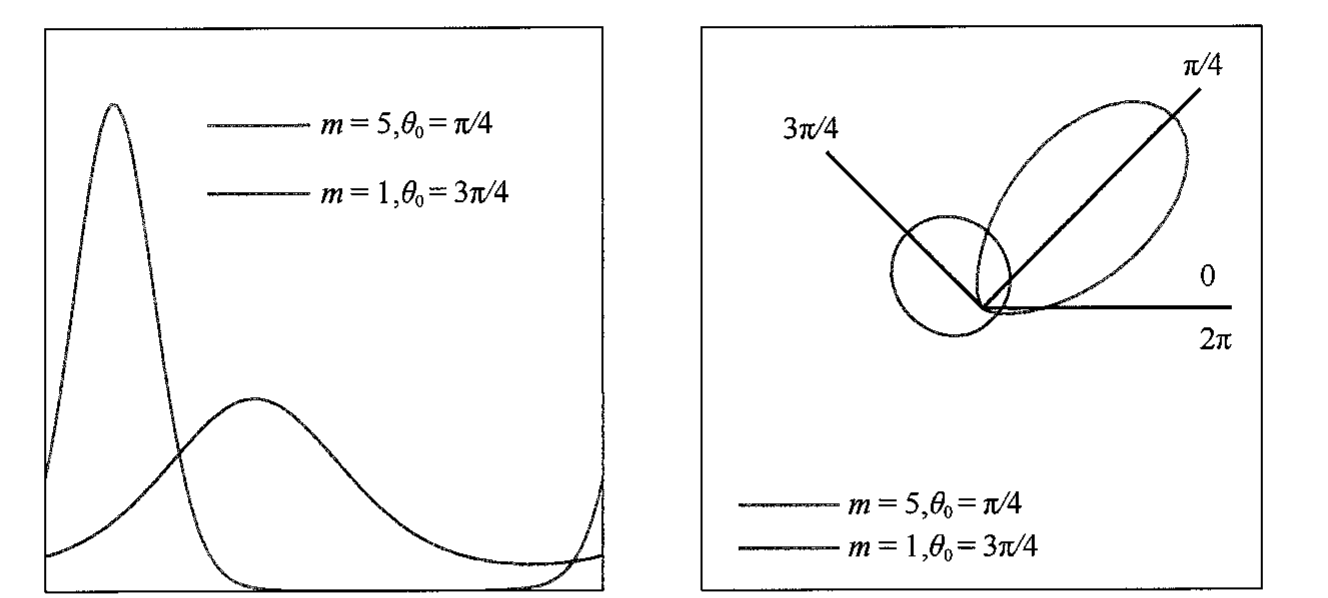
\includegraphics[width=0.82\textwidth]{ch03-fig3-11-vonmises.png}
  \caption{两个不同参数值下的 von Mises 分布。左图在笛卡儿坐标下，右图在相应的极坐标下。}
  \label{figure:ch03-冯米塞斯}
\end{figure}

\begin{figure}[htbp]
  \centering
  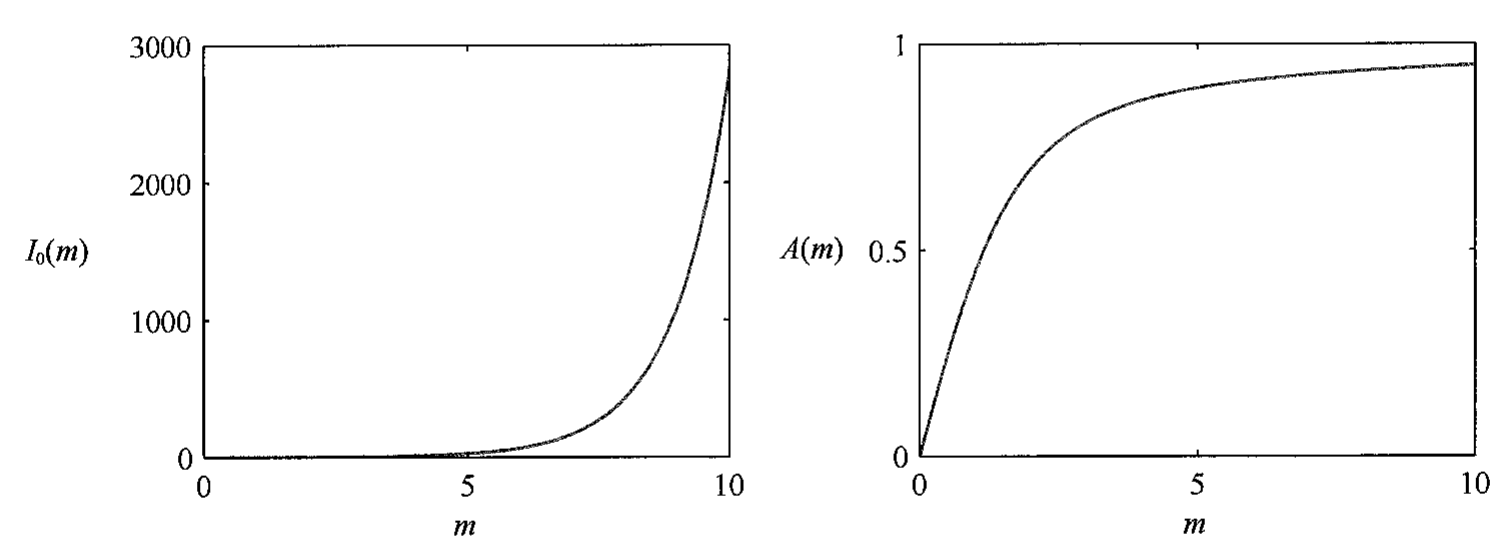
\includegraphics[width=0.82\textwidth]{ch03-fig3-12-bessel.png}
  \caption{Bessel 函数 $I_0(m)$（\eqref{align:ch03-修正Bessel函数}）和函数 $A(m)$（\eqref{align:ch03-Bessel比}）的图示。}
  \label{figure:ch03-Bessel函数}
\end{figure}

考虑 von Mises 分布中参数 $\theta_0$ 和 $m$ 的最大似然估计量。对数似然函数由下式给出：
\begin{align}
\ln p(\mathcal{D}\mid\theta_0,m)=-N\ln(2\pi)-N\ln I_0(m)+m\sum_{n=1}^{N}\cos(\theta_n-\theta_0).
\label{align:ch03-冯米塞斯对数似然}
\end{align}
令\eqref{align:ch03-冯米塞斯对数似然}对 $\theta_0$ 的导数为零，可得
\begin{align}
\sum_{n=1}^{N}\sin(\theta_n-\theta_0)=0.
\label{align:ch03-冯米塞斯驻点}
\end{align}
为了求解 $\theta_0$，使用如下三角恒等式：
\begin{align}
\sin(A-B)=\cos B\sin A-\cos A\sin B.
\label{align:ch03-正弦差}
\end{align}
由此可得（见\cref{exercise:ch03-32}）
\begin{align}
\theta_0^{\mathrm{ML}}=\tan^{-1}\!\left(\frac{\sum_n\sin\theta_n}{\sum_n\cos\theta_n}\right).
\label{align:ch03-冯米塞斯均值ML}
\end{align}
可以发现，这与之前二维笛卡儿空间中观测值均值的结果[\eqref{align:ch03-周期均值角}]一致。

类似地，关于 $m$ 最大化\eqref{align:ch03-冯米塞斯对数似然}，并利用 $I_0'(m)=I_1(m)$（Abramowitz and Stegun, 1965），可得
\begin{align}
A(m_{\mathrm{ML}})=\frac{1}{N}\sum_{n=1}^{N}\cos(\theta_n-\theta_0^{\mathrm{ML}}).
\label{align:ch03-聚焦参数ML}
\end{align}
此处已经代入了 $\theta_0$ 的最大似然解（注意我们现在正在对 $\theta$ 和 $m$ 进行联合优化），并定义了
\begin{align}
A(m)=\frac{I_1(m)}{I_0(m)}.
\label{align:ch03-Bessel比}
\end{align}
函数 $A(m)$ 如\cref{figure:ch03-Bessel函数}所示。利用\eqref{align:ch03-三角恒等式2}中的三角恒等式，可以将\eqref{align:ch03-聚焦参数ML}写成如下形式：
\begin{align}
A(m_{\mathrm{ML}})=\left(\frac{1}{N}\sum_{n=1}^{N}\cos\theta_n\right)\cos\theta_0^{\mathrm{ML}}+\left(\frac{1}{N}\sum_{n=1}^{N}\sin\theta_n\right)\sin\theta_0^{\mathrm{ML}}.
\label{align:ch03-聚焦参数展开}
\end{align}

\begin{proposition}[von Mises 分布的最大似然估计]\label{proposition:ch03-冯米塞斯最大似然}
设 $\theta_1,\cdots,\theta_N$ 为来自 von Mises 分布的独立观测，$N\geqslant1$。则 $\theta_0$ 的最大似然估计由\eqref{align:ch03-冯米塞斯均值ML}给出，$m$ 的最大似然估计满足\eqref{align:ch03-聚焦参数ML}，（二者合起来要求分母不为零）。
\end{proposition}
\begin{proof}
（重构新增）关于 $\theta_0$：对\eqref{align:ch03-冯米塞斯对数似然}求导，注意 $\frac{\mathrm{d}}{\mathrm{d}\theta_0}\cos(\theta_n-\theta_0)=\sin(\theta_n-\theta_0)$，得 $\partial\ln p/\partial\theta_0=m\sum_n\sin(\theta_n-\theta_0)$。令其为零（$m>0$）即得\eqref{align:ch03-冯米塞斯驻点}。

用\eqref{align:ch03-正弦差}展开\eqref{align:ch03-冯米塞斯驻点}：
\begin{align*}
\sum_n\sin(\theta_n-\theta_0)=\cos\theta_0\sum_n\sin\theta_n-\sin\theta_0\sum_n\cos\theta_n=0,
\end{align*}
于是 $\tan\theta_0=\dfrac{\sum_n\sin\theta_n}{\sum_n\cos\theta_n}$，按象限取分支即得\eqref{align:ch03-冯米塞斯均值ML}。这与\eqref{align:ch03-周期均值角}完全一致。

关于 $m$：对\eqref{align:ch03-冯米塞斯对数似然}求导，得
\begin{align*}
\frac{\partial\ln p}{\partial m}=-N\frac{I_0'(m)}{I_0(m)}+\sum_n\cos(\theta_n-\theta_0).
\end{align*}
令其为零并用 $I_0'(m)=I_1(m)$ 与 $A(m)=I_1(m)/I_0(m)$（\eqref{align:ch03-Bessel比}），得 $A(m_{\mathrm{ML}})=\frac1N\sum_n\cos(\theta_n-\theta_0^{\mathrm{ML}})$，即\eqref{align:ch03-聚焦参数ML}。

最后用\eqref{align:ch03-三角恒等式2}把 $\cos(\theta_n-\theta_0^{\mathrm{ML}})$ 展开即得\eqref{align:ch03-聚焦参数展开}。注意该式右端只依赖 $\theta_0^{\mathrm{ML}}$ 与数据，而 $A(m)$ 在 $(0,\infty)$ 上严格单调递增且值域为 $(0,1)$，故当右端落在 $(0,1)$ 内时 $m_{\mathrm{ML}}$ 唯一存在。
\end{proof}

% SUPPLEMENT: parent=proposition:ch03-冯米塞斯最大似然; kind=motivation; location=紧随其后的 remark（重构新增）
\begin{remark}（重构新增）
这里出现了一个漂亮的巧合：von Mises 分布的均值方向的最大似然估计，与“把观测当作单位圆上的向量再求平均”的圆周均值\eqref{align:ch03-周期均值角}完全相同。这解释了前面那句“读者很快就会看到这个结果是如何作为最大似然估计量而产生的”：圆周均值不是权宜之计，而是 von Mises 模型下的最大似然解。

$m$ 的估计则没有闭式解：\eqref{align:ch03-聚焦参数ML}只给出 $A(m_{\mathrm{ML}})$ 的值，需要数值反演 $A$ 才能得到 $m_{\mathrm{ML}}$（这正是\cref{figure:ch03-Bessel函数}右图的作用）。条件 $N\geqslant1$ 与分母 $\sum_n\cos\theta_n$、$\sum_n\sin\theta_n$ 不同时为零，保证 $\theta_0^{\mathrm{ML}}$ 有定义；若数据在圆周上完全均匀，则 $\sum_n\cos\theta_n=\sum_n\sin\theta_n=0$，均值方向不可辨识，此时 $m_{\mathrm{ML}}=0$ 对应均匀分布。
\end{remark}

\eqref{align:ch03-聚焦参数展开}的右侧部分很容易计算，而函数 $A(m)$ 可以通过数值反演得到。von Mises 分布的一个局限性是，它是单峰的。我们可以通过构造一个包含多个 von Mises 分布的混合分布来获得一个更为灵活的周期变量建模框架，以处理多峰数据。

为了讨论的完整性，下面简要提及一些构造周期分布的替代技术。最简单的方法是使用观测值的直方图，其中角坐标被划分为固定的区间。这种方法的优点是简单且灵活，但也存在显著的局限性，这一点读者在后文对直方图方法的详细讨论中将会看到（参见\cref{subsection:ch03-直方图}）。另一种方法类似于 von Mises 分布：从欧氏空间上的 Gauss 分布开始，但现在边缘化到单位圆上，而不是条件化（Mardia and Jupp, 2000）。然而，这会导致分布形式更加复杂，因此我们不再做进一步讨论。最后，实轴上的任何有效分布（如 Gauss 分布）都可以通过将宽度为 $2\pi$ 的连续区间映射到周期变量 $(0,2\pi)$ 上，成为周期分布，这相当于将实轴“包裹”到单位圆上（环绕分布）。同样，由此得到的分布比 von Mises 分布更复杂。

\begin{remark}（重构新增）
这段列举了三种替代构造，它们分别对应三种“把直线上的工具搬到圆周上”的思路：直方图法直接对角度分箱，不做参数假设；边缘化法把平面 Gauss 分布的 $r$ 积分掉，得到圆周上的边缘密度（其形式不再是 von Mises）；包裹法把实轴按 $2\pi$ 取模卷到圆上，得到“环绕”分布（如包裹正态分布）。

选择哪种构造取决于问题：若只需快速可视化，直方图足够；若需要解析上可处理的单峰模型，von Mises 最方便；若数据可能多峰，则应使用 von Mises 混合模型。所有这些构造的共同点是它们都满足\eqref{align:ch03-周期分布非负}至\eqref{align:ch03-周期分布周期}，区别只在于密度的具体形式与计算复杂度。
\end{remark}

\end{document}
